% !TeX encoding = UTF-8
% !TeX root = master.tex
% !TeX spellcheck = en_US

\documentclass[11pt,a4paper,twoside,openright]{report}

\usepackage[utf8]{inputenc}
\usepackage[portuguese,english]{babel}
\selectlanguage{english}

\usepackage[mieic]{styles/feupteses}
% Additional options for feupteses.sty:
% - juri: prints line numbers
% - final: final version
% - onpaper: links are not shown (for paper versions)
% - backrefs: include back references from bibliography to citation place

%\usepackage[lofdepth,lotdepth]{subfig}
\usepackage{afterpage}
\usepackage{graphicx}
\usepackage{flafter}
\usepackage{animate}
\usepackage{float}
\usepackage{grffile}

\usepackage{color}
\definecolor{cloudwhite}{cmyk}{0,0,0,0.025}

\usepackage{listings}
\lstset{ %
 language=C++,                        % choose the language of the code
 basicstyle=\footnotesize\ttfamily,
 keywordstyle=\bfseries,
 numbers=left,                      % where to put the line-numbers
 numberstyle=\scriptsize\texttt,    % the size of the fonts that are used for the line-numbers
 stepnumber=1,                      % the step between two line-numbers. If it's 1 each line will be numbered
 numbersep=8pt,                     % how far the line-numbers are from the code
 frame=tb,
 float=htb,
 aboveskip=8mm,
 belowskip=4mm,
 backgroundcolor=\color{cloudwhite},
 showspaces=false,                  % show spaces adding particular underscores
 showstringspaces=false,            % underline spaces within strings
 showtabs=false,                    % show tabs within strings adding particular underscores
 tabsize=2,	                    % sets default tabsize to 2 spaces
 captionpos=b,                      % sets the caption-position to bottom
 breaklines=true,                   % sets automatic line breaking
 breakatwhitespace=false,           % sets if automatic breaks should only happen at whitespace
 escapeinside={\%*}{*)},            % if you want to add a comment within your code
 morekeywords={*,var,template,new}  % if you want to add more keywords to the set
}

\usepackage{amsmath}
\usepackage[algochapter,linesnumberedhidden]{algorithm2e}
\usepackage{booktabs}
\usepackage{tabu}
\usepackage{rotating}
\usepackage{array}
\usepackage{multirow}
\usepackage{easylist}
\usepackage{siunitx}
\usepackage{url}
\usepackage{caption}
\usepackage{subcaption} 
\usepackage{footnote}
\usepackage{footmisc}
\usepackage{hyperref}
\usepackage[all]{hypcap}
\usepackage[noabbrev,nameinlink]{cleveref}
\usepackage{etoolbox}
\usepackage[nonumberlist,acronym,xindy]{glossaries}

\usepackage{enumitem}
\setlist{nolistsep}

\graphicspath{{figures/}}
\setcounter{tocdepth}{3}

\makeglossaries
%\usepackage[xindy]{imakeidx}
%\makeindex


\newtoggle{showcommittee}
\toggletrue{showcommittee}

%some macro definitions

% format
\newcommand{\class}[1]{{\normalfont\slshape #1\/}}

% entities
\newcommand{\Feup}{Faculdade de Engenharia da Universidade do Porto}

% abbreviations:
\newacronym{agps}{AGPS}{Assisted Global Positioning System}
\newacronym{amcl}{AMCL}{Adaptive Monte Carlo Localization}
\newacronym{api}{API}{Application Programming Interface}
\newacronym{cad}{CAD}{Computer Aided Design}
\newacronym{carlos}{CARLoS}{Cooperative Autonomous Robot for Large Open Spaces}
\newacronym{dof}{DoF}{Degrees of Freedom}
\newacronym{dgps}{DGPS}{Differential Global Positioning System}
\newacronym{ekf}{EKF}{Extended Kalman Filter}
\newacronym{esf}{ESF}{Ensemble of Shape Functions}
\newacronym{fpfh}{FPFH}{Fast Point Feature Histogram}
\newacronym{glonass}{GLONASS}{GLObalnaya NAvigatsionnaya Sputnikovaya Sistema}
\newacronym{gnss}{GNSS}{Global Navigation Satellite System}
\newacronym{gps}{GPS}{Global Positioning System}
\newacronym{gpu}{GPU}{Graphics Processing Unit}
\newacronym{icp}{ICP}{Iterative Closest Point}
\newacronym{ip}{IP}{Internet Protocol}
\newacronym{iss3d}{ISS3D}{3D Intrinsic Shape Signatures}
\newacronym{lidar}{LIDAR}{LIght Detection And Ranging}
\newacronym{mcl}{MCL}{Monte Carlo Localization}
\newacronym{ndt}{NDT}{Normal Distributions Transform}
\newacronym{opencv}{OpenCV}{Open Computer Vision library}
\newacronym{openni}{OpenNI}{Open Natural Interaction library}
\newacronym{pca}{PCA}{Principal Component Analysis}
\newacronym{pcl}{PCL}{Point Cloud Library}
\newacronym{pfh}{PFH}{Point Feature Histogram}
\newacronym{radar}{RADAR}{RAdio Detection And Ranging}
\newacronym{ransac}{RANSAC}{Random Sample Consensus}
\newacronym{ros}{ROS}{Robot Operating System}
\newacronym{rmse}{RMSE}{Root Mean Square Error}
\newacronym{sacia}{SAC-IA}{Sample Consensus Initial Alignment}
\newacronym{sc3d}{SC3D}{Shape Context 3D}
\newacronym{shot}{SHOT}{Signature of Histograms of Orientations}
\newacronym{sift}{SIFT}{Scale Invariant Feature Transform}
\newacronym{slam}{SLAM}{Simultaneous Localization And Mapping}
\newacronym{sonar}{SONAR}{SOund Navigation And Ranging}
\newacronym{tcp}{TCP}{Transmission Control Protocol}
\newacronym{toa}{ToA}{Time of Arrival}
\newacronym{tof}{ToF}{Time of Flight}
\newacronym{ttff}{TTFF}{Time To First Fix}
\newacronym{udp}{UDP}{User Datagram Protocol}
\newacronym{ukf}{UKF}{Unscented Kalman Filter}
\newacronym{usc}{USC}{Unique Shape Context}
\newacronym{xml}{XML}{Extensible Markup Language}
\newacronym{xmlrpc}{XML-RPC}{Extensible Markup Language Remote Procedure Call}

% nomenclature:
%\newglossaryentry{label}{name=$symbol$, description={multi line description}}



\begin{document}


%---------------------------------------------------------------------------------------------------
% Top matter | Information about author, supervisors and committee
%---------------------------------------------------------------------------------------------------

\title{Robot Self-Localization in Dynamic Environments}
\author{Carlos Miguel Correia da Costa}
\thesisdate{January 26, 2015}
\copyrightnotice{Carlos Miguel Correia da Costa, 2015}
\supervisor{Supervisor}{Armando Jorge Miranda de Sousa (Ph.D.)}
\supervisor{Second Supervisor}{Germano Manuel Correia dos Santos Veiga (Ph.D.)}

\iftoggle{showcommittee} {
	\committeetext{Approved in oral examination by the committee:}
	\committeemember{Chair}{Doctor Name of the President}
	\committeemember{External Examiner}{Doctor Name of the Examiner}
	\committeemember{Supervisor}{Doctor Name of the Supervisor}
	\signature
}

\logo{uporto-feup.pdf}



%---------------------------------------------------------------------------------------------------
% Prolog
%---------------------------------------------------------------------------------------------------

\begin{Prolog}
  \chapter*{Abstract}

Mobile robot platforms capable of operating safely and accurately in dynamic environments can have a multitude of applications, ranging from simple delivery tasks to advanced assembly operations. These abilities rely heavily on a robust navigation stack, which requires a stable and accurate localization system.

This dissertation describes an efficient, modular, extensible and easy to configure 3/6 DoF localization system, capable of operating on a wide range of mobile robot platforms and environments. It is able to reliably estimate the global position using feature matching and is capable of achieving high accuracy pose tracking using point cloud registration algorithms. It can use several point cloud sensing devices (such as LIDARs or RGB-D cameras) and requires no artificial landmarks. Moreover, it can update the localization map at runtime and dynamically adjust its operation rate based on the predicted robot velocity in order to use the minimum amount of hardware resources. It also offers a detailed analysis of each pose estimation, providing information about the percentage of registered inliers, the root mean square error of the inliers, the angular distribution of the inliers and outliers, the pose corrections that were performed in relation to the expected position and in case of initial pose estimation it also gives the distribution of the acceptable initial poses, which can be very valuable information for a navigation supervisor when the robot is in ambiguous areas that are very similar in different parts of the known environment.

The ROS implementation was tested in several dynamic indoor environments using two mobile robot platforms equipped with LIDARs and RGB-D cameras. Overall tests using sensor data from simulation and retrieved from the robot platforms performed in a high end laptop with an Intel Core i7 3630QM processor, 16GB DDR3 of memory and NVIDIA GTX680M graphics card, demonstrated high accuracy in complex dynamic environments, with less than 1 cm in translation error and less than 1 degree in rotation error. Execution times ranged from 5 to 30 milliseconds in a 3 DoF setup and from 50 to 150 milliseconds in a full dynamic 6 DoF configuration.

The sub centimeter accuracy achieved by the proposed localization system along with the dynamic map update capability and the need of no artificial landmarks will allow the fast deployment of mobile robot platforms capable of operating safely and accurately in cluttered environments. Moreover, the resilience to dynamic objects will grant the possibility to use robots as coworkers, helping humans perform their work more efficiently and thus reducing the overall production costs.



\chapter*{Resumo}

\begin{otherlanguage}{portuguese}

Plataformas móveis robóticas capazes de operar com precisão e de forma segura em ambientes dinâmicos têm um alargado espetro de aplicações, desde simples entregas de objetos até operações complexas de montagem. Para atingir estes requisitos de operação é necessário um sistema de navegação robusto, que por sua vez requer um módulo de localização preciso e estável.

Esta dissertação descreve um sistema de localização 3/6 DoF eficiente, modular, extensível e fácil de configurar, capaz de operar num alargado conjunto de plataformas móveis e ambientes. É capaz de estimar a posição inicial de um robô usando métodos de associação de características geométricas e consegue seguir a sua pose com alta precisão através de algoritmos de registo de nuvens de pontos. A sua implementação consegue tirar partido de vários sensores laser e câmaras RGB-D e não necessita de marcadores artificiais ou modificação do ambiente. Possui ainda a capacidade de atualizar o mapa incrementalmente e ajustar a sua frequência de funcionamento de acordo com a velocidade do robô de forma a usar o mínimo de recursos computacionais possível. Para facilitar a avaliação da qualidade da localização para operações críticas, cada estimativa da pose do robô é acompanhada com a análise do registo da nuvem de pontos, contendo informação acerca da percentagem de pontos corretamente registados, a raiz quadrada do erro quadrático médio, a distribuição angular dos pontos classificados como pertencentes e não pertencentes ao mapa de referência, as correções aplicadas à estimativa da pose e no caso de ser efetuada localização global também é disponibilizada a distribuição das poses iniciais aceitáveis, o que pode ser informação bastante útil para um supervisor de navegação quando o robô está em posições ambíguas do ambiente nas quais existe geometria semelhante em sítios diferentes do mapa.

A implementação em ROS foi testada em vários ambientes dinâmicos recorrendo a duas plataformas móveis equipadas com LIDARs e câmaras RGB-D. Os resultados obtidos usando dados de simulação e recolhidos das plataformas robóticas realizados num portátil com CPU Intel Core i7 3630QM, 16GB DDR3 de memória e placa gráfica NVIDIA GTX680M demonstraram que o sistema consegue fazer a estimativa da pose do robô com um erro de translação inferior a 1 centímetro e um erro de rotação abaixo de 1 grau. Os tempos de execução oscilaram entre 5 e 30 milissegundos para uma configuração 3 DoF e entre 50 e 150 milissegundos para 6 DoF.

A alta precisão disponibilizada pelo sistema de localização proposto em conjunto com a sua capacidade para atualizar o mapa incrementalmente e de não necessitar marcadores artificiais, irá permitir o desenvolvimento de plataformas robóticas móveis capazes de operar em ambientes não estruturados. Por outro lado, a sua robustez em relação a objetos dinâmicos abre a possibilidade dos robôs colaborarem com humanos para melhorar a produtividade global de uma dada tarefa e assim reduzir os custos de produção.

\end{otherlanguage}

  \chapter*{Acknowledgments}

I would like to express my gratitude to my supervisors and the INESC team, for their helpful contributions. Their experience and expertise significantly improved the quality of this dissertation.

I am also very grateful for the knowledge and experiences that I gather from my friends, teachers and colleagues over the years and for the brilliant work developed by the ROS and PCL community.

And of course, to my family, for their continuous support.

\vspace{10mm}
\flushleft{Carlos Miguel Correia da Costa}

  \cleardoublepage
\thispagestyle{plain}

\vspace*{8cm}

\begin{flushright}
  \textsl{``Perfection is achieved, not when there is nothing more to add, \\
           but when there is nothing left to take away.''} \\
  \vspace*{1.5cm}
           Antoine de Saint-Exupéry
\end{flushright}

  \cleardoublepage
  \pdfbookmark[0]{Table of Contents}{contents}
  \tableofcontents
  \cleardoublepage
  \pdfbookmark[0]{List of Figures}{figures}
  \listoffigures
  \cleardoublepage
  \pdfbookmark[0]{List of Tables}{tables}
  \listoftables
  \listofalgorithms
%  \glsaddall
  \printglossary[type=\acronymtype,title=Abbreviations]
  \printglossary[title=Nomenclature]
\end{Prolog}



%---------------------------------------------------------------------------------------------------
% Chapters
%---------------------------------------------------------------------------------------------------

\StartBody

\chapter{Introduction} \label{chap:introduction}



\section*{}

This chapter provides an overview about the motivations and objectives of this dissertation along with its practical applications.



\section{Context}\label{sec:introduction_context}

Humanity has sought a reliable method of navigation ever since it started to explore the world. It began with simple landmark reference points for local travels, then perfected celestial navigation for global journeys, and when it finally conquered space, it deployed a global system for high accuracy localization. Autonomous robots face the same problem, because in order to be able to navigate with precision, they first need to know their location.

Over the years, several localization methods have been proposed and refined, according to the navigation environment and the accuracy requirements. Some are meant for high precision local navigation, while others provide an approximate global position.

A robot capable of operating safely and accurately in a dynamic environment can have innumerous applications, ranging from simple delivery tasks to advanced assembly. Besides improving productivity by performing repetitive tasks with precision and speed, robots can also act as coworkers, helping humans perform their jobs more efficiently and thus, reducing the overall production costs.



\section{Project}\label{sec:introduction_project}

\gls{carlos}\footnote{\url{http://carlosproject.eu/}} is a European research project that aims to develop an autonomous robot capable of performing repetitive tasks alongside human co-workers in dynamic environments. The robot will operate in shipyards and is intended to perform fit-out operations, such as stud welding and projection mapping of \gls{cad} drawings. Stud welding is a repetitive task that provides structural support for other components, such as heat insulation layers or electrical systems. Projection mapping of \gls{cad} drawings or other important information will help human co-workers assemble components faster, because it will mark the exact position in which they must be installed.



\section{Motivation and objectives}\label{sec:introduction_goals}

With the increase of competitiveness in the current globalized trading markets, companies are trying to reduce production costs and improve the productivity of their assets. Robots can help achieve these goals by performing the simple and repetitive jobs while giving humans more free time to perform the complex and creative tasks.

Mobile platforms equipped with robotic arms provide a flexible way to automate a wide range of tasks that must be performed over large areas. However, before performing the intended operations they first need to know where they are and how they can reach the desired location. Moreover, given their limited computational resources and energy storages, they require efficient, reliable and accurate control systems capable to operate in real time.



\section{Contributions}\label{sec:introduction_contributions}

This dissertation introduces an efficient, modular and extensible 3/6 \gls{dof} localization system for mobile robot platforms capable of operating accurately and reliably in dynamic environments. It is a multi-level registration pipeline that uses geometric features to estimate the initial position of a robot platform and point cloud registration algorithms to track its pose. The tracking subsystem can have two different configurations. One tuned for maximum efficiency used for the normal operation of the mobile platform and another for unlikely situations that may require more robust registration algorithms / configurations. It also supports incremental map update and can adjust its operation rate based on the estimated robot velocity. For critical operations, it provides a detailed analysis of the tracking quality and when initial pose estimation is required it gives the distribution of the acceptable poses, which can be very valuable information if there are several areas in the known map with very similar geometry.



\section{Dissertation outline}\label{sec:introduction_structure}

The remaining of this dissertation is split over 5 chapters. \Cref{chap:localization-methods} provides an overview of the main localization methods available for mobile robot platforms. \Cref{chap:relevant-sofware-technologies} introduces the main frameworks used to implement the self-localization system. \Cref{chap:localization-system} details the architecture and \gls{ros} implementation of the proposed 3/6 \gls{dof} self-localization system. \Cref{chap:localization-system-evaluation} evaluates the results achieved with the localization system in several testing environments. Finally, \cref{chap:conclusions-and-future-work} presents the conclusions of this dissertation and suggestions for future work.

\chapter{Localization methods}\label{chap:localization-methods}



\section*{}

Self-localization is critical to any autonomous robot that must navigate the environment and requires the calculation of a 3/6 \gls{dof} pose in a given world coordinate system.

Over the years, several approaches were developed according to the precision requirements and the environment in which the robot is designed to operate. Some require support systems to calculate the position, while others are completely autonomous, allowing the robot to localize itself without any outside dependencies. Also, some systems have limited range while others can only be effective in open spaces. Moreover, several of these methods were designed to cope with errors in the localization sensors and tolerate temporary malfunctions.

The following sections will introduce some of the most used self-localization systems that can be employed in the estimation of a robot's pose.



\section{Proprioceptive methods}

Proprioceptive methods rely on internal information that the robot possesses about its own systems operation and movement in order to update the current pose estimation. As a result, they allow the robot to operate without an external support system.

Since these methods don't correct their estimations based on environment observations, they are bound to have significant cumulative errors. As such, in order to maintain an accurate estimation of a robot's pose, they are usually combined with exteroceptive systems.


\subsection{Odometry}

Odometry estimates the current pose by integrating the velocity of the robot over time. This velocity is usually calculated by measuring the number of rotations of the wheels (using optical encoders like the ones shown in \cref{fig:localization-methods_optic-encoders}). This method can provide a viable approximated location, as can be seen in \cite{Reinstein2013}.

\afterpage{
\begin{figure}[H]
	\centering
	\includegraphics*[width=0.5\textwidth]{localization_methods/optic_encoders}
	\caption[Different types of optical encoders used to measure distances]{Different types of optical encoders used to measure distances\protect\footnotemark}
	\label{fig:localization-methods_optic-encoders}
\end{figure}
\footnotetext{\url{http://www.mindspring.com/~tom2000/Delphi/Codewheel.html}}
}


\subsection{Dead reckoning}

Dead reckoning is an extension of the odometry method, in which the acceleration and angular velocity are used to improve the localization estimations.

Other sensors, such as accelerometers and gyroscopes, can also be used to improve the position estimation \cite{Ibraheem2010} and provide the robot orientation.



\section{Exteroceptive methods}

Exteroceptive methods use a range of sensors to analyze the environment and retrieve the necessary information to perform localization.


\subsection{Trilateration methods}

Trilateration is a geometric technique that can be employed in the calculation of absolute or relative positions using distances from known points.

For 3D localization, it usually involves the intersection of 4 or more spheres, in which their radius is the distance to known positions.


\subsubsection{\glsentryfirst{gnss}}

\gls{gnss} such as the \gls{gps} or \gls{glonass}, allow 3D positioning in the planet Earth  using a trilateration method \cite{Knedlik2007}.

In these systems, a constellation of satellites broadcasts a radio signal with information about its position along with the time of the message dispatch. Using this data and knowing the speed of the radio waves, the distances to the satellites can be computed.

With at least 3 satellites distances, the 3D position can be calculated, since the Earth can be used as the ${4}^{th}$ sphere (\cref{fig:localization-methods_gnss} shows a visual representation of the trilateration technique used in a global localization system).

Given that the correct measurement of the distances to the satellites relies in the accurate computation of the elapsed time between the message dispatch and its reception, it is critical that both the satellites and the receiver have synchronized clocks. This is achieved by using high precision atomic clocks in the satellites and a clock reset technique in the receiver. This reset method relies on the fact that 3 satellite distances will only have a valid location if the clock of the receiver is synchronized. With this knowledge, the receiver can compute the necessary corrections to reset its internal clock to match the satellites time.

%\afterpage{
\begin{figure}[H]
	\centering
	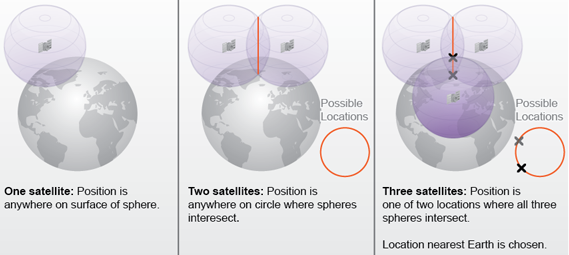
\includegraphics[width=0.8\textwidth]{localization_methods/gnss}
	\caption[Trilateration technique in a global localization system]{Trilateration technique in a global localization system\protect\footnotemark}
	\label{fig:localization-methods_gnss}
\end{figure}
\footnotetext{\url{https://www.e-education.psu.edu/geog160/node/1923}}
%}


\subsubsection{\glsentryfirst{dgps}}

The accuracy of the \gls{gps} position can be increased with the help of local broadcast stations. These stations are fixed and provide information about the corrections that can be made to the satellite signals in order to improve the localization precision.

These corrections are useful to mitigate some of the ambient interference that the satellite signals face. These interferences can range from simple signal reflection in the environment landscape to the more complex interactions with the atmosphere, which can change the speed and path of the radio signals.

The computation of the corrections \cite{Kim2007} is based on the fact that these stations are fixed, and as such, they can compare the location given by the satellite signals with their known location. With this position differential, the appropriate corrections can be calculated and broadcasted to the \gls{gps} receivers.


\subsubsection{\glsentryfirst{agps}}

\gls{agps} systems are a common method used to speed up the \gls{ttff} of a \gls{gps} receiver. They usually rely on the cellphone network to provide location estimation and signal corrections \cite{R.1948}. This information can greatly reduce the \gls{ttff} when there are few satellites visible or their signal is very weak and only temporary available.


\subsubsection{Signal strength geolocation methods}

Signal strength geolocation \cite{Kobayashi2002}, also known as fingerprinting localization \cite{Bshara2010}, is an approximate method that can be used to calculate relative positions.

It relies on the analysis of the signal attenuation from a given access point (like a Wi-Fi router or cellphone tower), to estimate distances. With enough access points (usually 4), an approximate position can be computed.

This type of distance estimation can be useful for indoor navigation, but requires a propagation model of the signal and the environment. If these models aren't accurate, then the localization precision of these methods will be very low.

Although this method is less accurate than the more recent global localization systems (such as \gls{gps}), it can be used without human made infrastructures, and as such, is a viable solution in case of temporary disruption of the \gls{gps} signal.


\subsection{Celestial navigation}

Celestial navigation \cite{Yang2011} relies on the observation of stars, planets or other reference objects, to calculate the latitude and longitude.

The calculation of the position on the surface of the Earth using celestial navigation is similar to trilateration, but in this case, angles are used instead of distances. These angles (delta), are measured between the Earth horizon and the center of the celestial object.

Having the delta, and knowing the relative position of the Earth to the reference object, along with the Greenwich hour time, it is possible to calculate a circle of position (as shown in \cref{fig:localization-methods_celestial-navigation}).

Having at least 3 circles of position, the latitude and longitude can be computed.

Although this method is less accurate than the more recent global localization systems (such as \gls{gps}), it can be used without human made infrastructures, and as such, is a viable solution in case of temporary disruption of the \gls{gps} signal.

%\afterpage{
\begin{figure}[H]
	\centering
	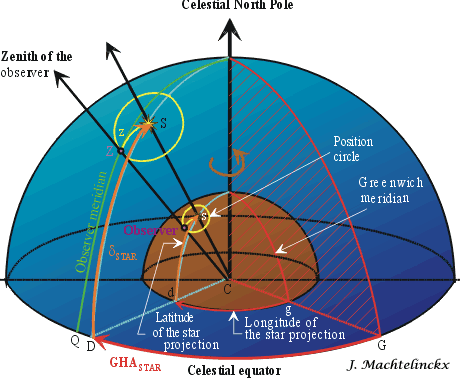
\includegraphics[width=0.45\textwidth]{localization_methods/celestial_navigation}
	\caption[Circle of position in celestial navigation]{Circle of position in celestial navigation\protect\footnotemark}
	\label{fig:localization-methods_celestial-navigation}
\end{figure}
\footnotetext{\url{http://onboardintelligence.com/CelestialNav/Celnav2.aspx}}
%}


\subsection{Landmark methods}

Landmark methods \cite{Lee2006} can be used to perform relative localization, and are very useful to reduce the required information for navigation.

In these methods a database of markers / environment geometry is stored along with its location, and when the robot recognizes one of these markers, it corrects its proprioceptive methods measures.

It is a simplification of the method that will be presented in the next section, and it is useful for environments that have unique geometry in key positions of the navigation map.


\subsection{Point cloud methods}

Point cloud localization methods can be used to perform relative localization by finding the best point cloud match between the environment and the know map (\cref{fig:localization-methods_icp} shows its application to small objects). These methods require a 2D or 3D representation of the environment and tend to be used in conjunction with proprioceptive methods (to have an estimation of movement), and also with probabilistic methods (when the point cloud acquisition location is not known).

One of the most used algorithms for 3D point cloud matching is the \gls{icp} \cite{Besl1992,Jez2008,Zhang1992,Bouaziz2013,Chetverikov2002,Djehaich2013,Zhou2011}. It is an iterative algorithm that finds the translation and rotation transformations that minimizes the distances of the corresponding points on both clouds.

There are several variants that optimize different parts of the algorithm \cite{Rusinkiewicz2001}.

The main steps for each iteration of \gls{icp} algorithm are presented below.

\begin{enumerate}
	\item  Selection of points in one or both point clouds (source and reference clouds)
	\item  Matching / pairing source points to reference points
	\item  Weighting the corresponding pairs
	\item  Rejecting low quality matches (outliers)
	\item  Assigning an error metric based on the point pairs
	\begin{enumerate}
		\item  Usually mean square error based on points distance
	\end{enumerate}
\end{enumerate}


%\afterpage{
\begin{figure}[H]
	\centering
	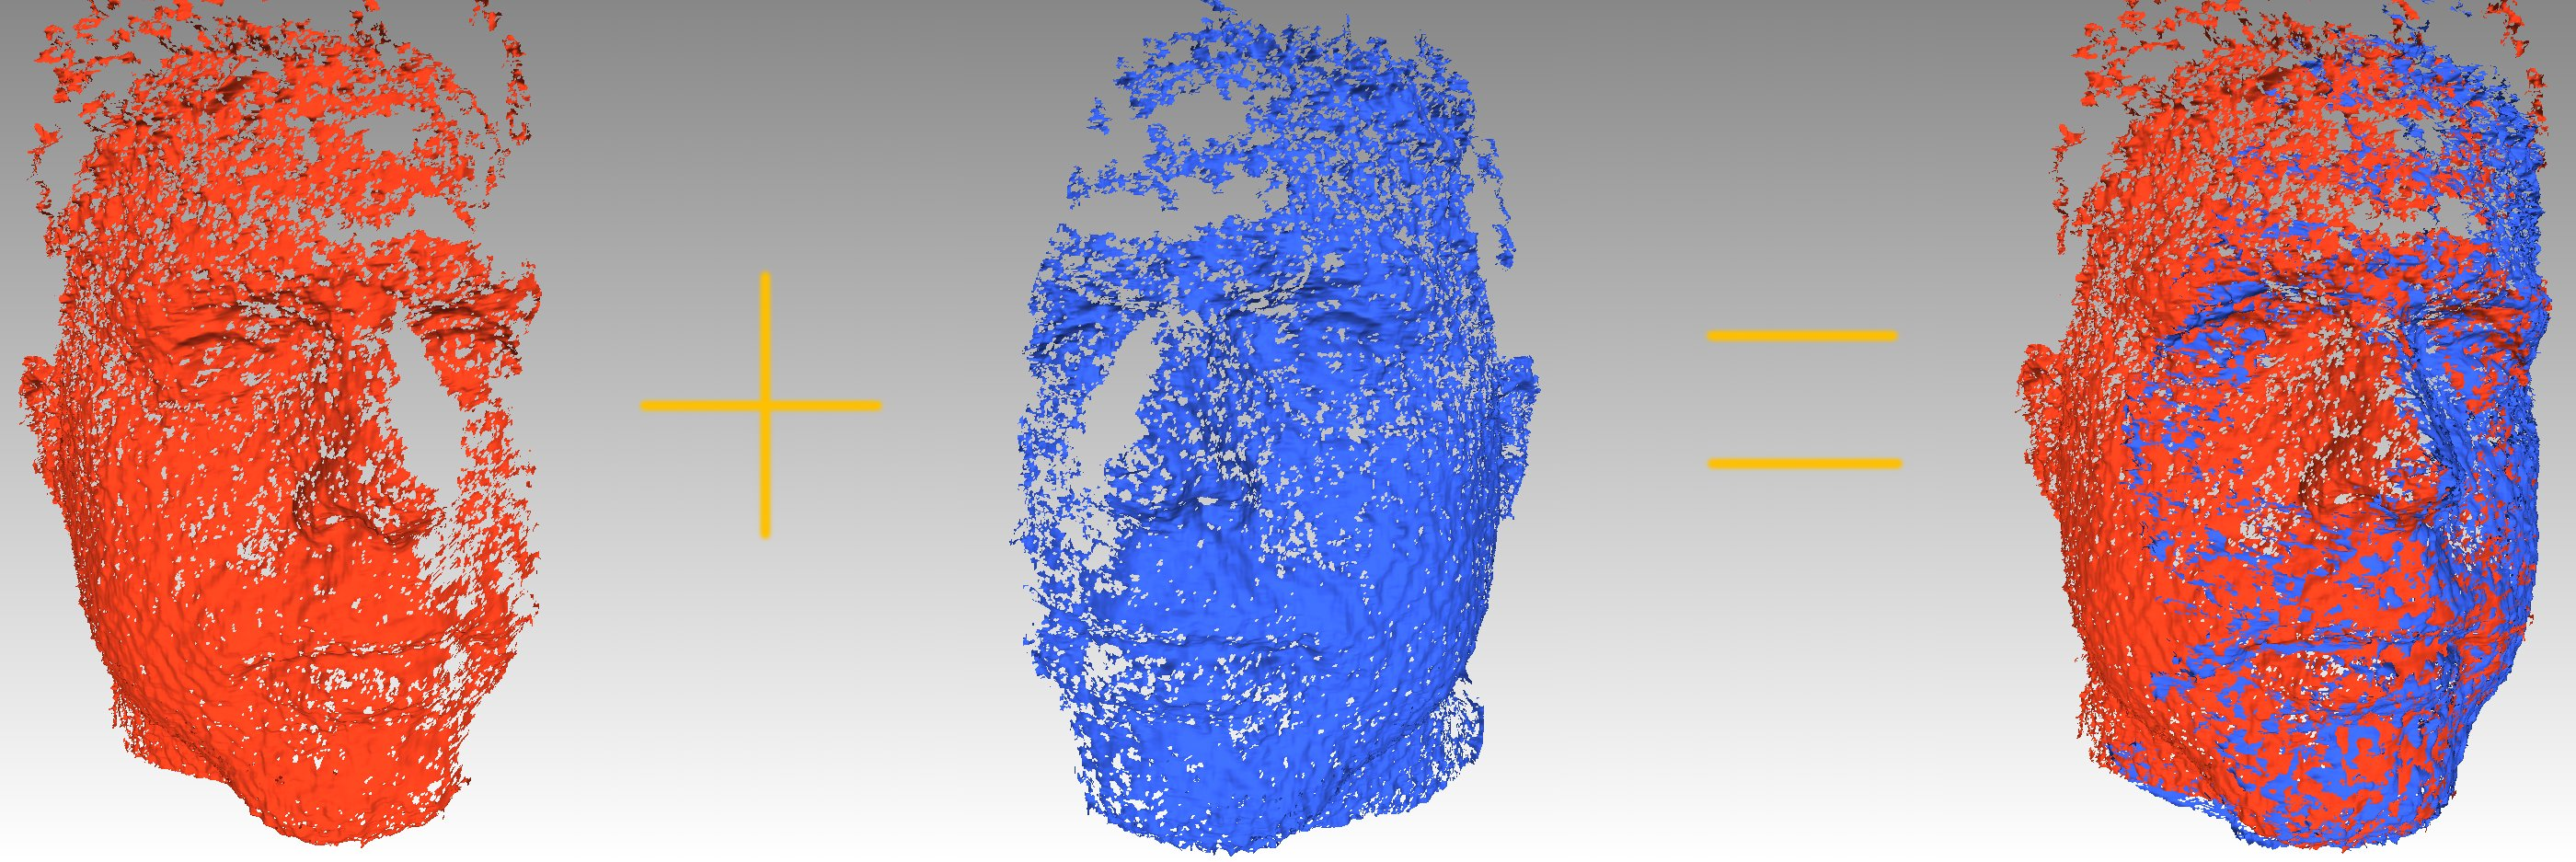
\includegraphics[width=0.75\textwidth]{localization_methods/icp}
	\caption[\glsentrytext{icp} point cloud matching]{\glsentrytext{icp} point cloud matching\protect\footnotemark}
	\label{fig:localization-methods_icp}
\end{figure}
\footnotetext{\url{http://dynface4d.isr.uc.pt/database.php}}
%}


\subsection{Probabilistic methods}

Probabilistic methods aim to reduce the impact of sensor accumulated errors or even temporary malfunctions by using Bayesian estimations and Markov processes.


\subsubsection{\glsentryfirst{mcl}}

\gls{mcl} (also known as particle filter), is a global localization algorithm that estimates the position and orientation of a robot by analyzing and adjusting the distribution and weights of state particles on a given environment \cite{Bshara2010,Arulampalam2002,Blanco2010,Chen2003b,Fox1999,Saito2009}.

It starts by randomly distributing the state particles on the map, and over time it changes their position and weight according to new sensor readings. The probable location of the robot will be in the area of the map that has the largest cluster of state particles. The figures below show the evolution of the state particles distribution during the robot movement in the environment, and illustrates how the new sensor readings changed the particles clusters\footnote{\url{http://www.cs.washington.edu/robotics/mcl/}}.

\begin{figure}[H]
	\centering
	\begin{minipage}[h]{.49\textwidth}
		\centering
		\animategraphics[width=\textwidth,loop,autoplay]{4}{localization_methods/mcl/frame-}{0}{39}
		\caption{\glsentrytext{mcl} particle distribution animation}
		\label{fig:localization-methods_mcl1}
	\end{minipage}\hfill
	\begin{minipage}[h]{.49\textwidth}
		\centering
		\includegraphics*[width=\textwidth]{localization_methods/mcl_2}
		\caption{\glsentrytext{mcl} redistribution of particles}
		\label{fig:localization-methods_mcl2}
	\end{minipage}
\end{figure}

\begin{figure}[H]
	\centering
	\begin{minipage}[h]{.49\textwidth}
		\centering
		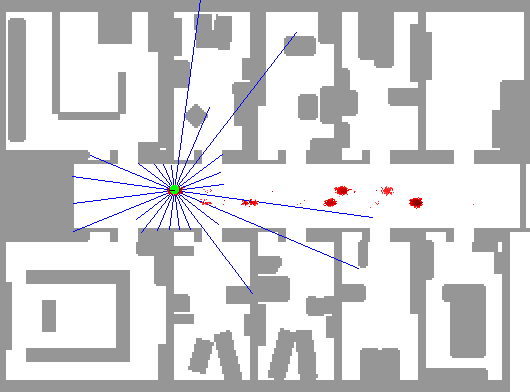
\includegraphics[width=\textwidth]{localization_methods/mcl_3}
		\caption{\glsentrytext{mcl} position refinement}
		\label{fig:localization-methods_mcl3}
	\end{minipage}\hfill
	\begin{minipage}[h]{.49\textwidth}
		\centering
		\includegraphics*[width=\textwidth]{localization_methods/mcl_4}
		\caption{\glsentrytext{mcl} position estimation}
		\label{fig:localization-methods_mcl4}
	\end{minipage}
\end{figure}


\subsubsection{Kalman filters}

Kalman filters \cite{Kalman1960} are probabilistic algorithms that estimate a given system state even when it is affected by noise or other errors. They perform linear quadratic estimations to achieve optimal results and can be efficiently implemented to be used in real time systems. They are recursive algorithms based on Marcov processes, and as a result, they only need to know the current system state in order to perform measurement corrections.

The \gls{ekf} \cite{Einicke1999,Ribeiro2004,Ivanjko2010,Liu2011} is a variant of the Kalman filter, designed to handle non-linear systems by performing linear approximations to the state variables. These approximations may lead to divergence in the estimations, and as such, the \gls{ekf} can't guarantee optimal results.

The \gls{ukf} \cite{Julier1997,Wan2002} is another variant of the Kalman filter that was designed for highly non-linear systems. It usually achieves better results than \gls{ekf} due to its unscented transform.

For the particular case of localization, these algorithms start with an initial estimation of the system state, and for each new position (computed from the sensors data), they predict the estimated robot location (according to the Bayes estimation model and the Gaussian distribution of errors), and then update their internal model of the system (mean and covariance) to incorporate the system evolution.

In \cref{fig:localization-methods_ukf} can be seen that the \gls{ukf} estimated position (red) is closer to the real position (blue) than the raw sensor measurements (green).

%\afterpage{
\begin{figure}[H]
	\centering
	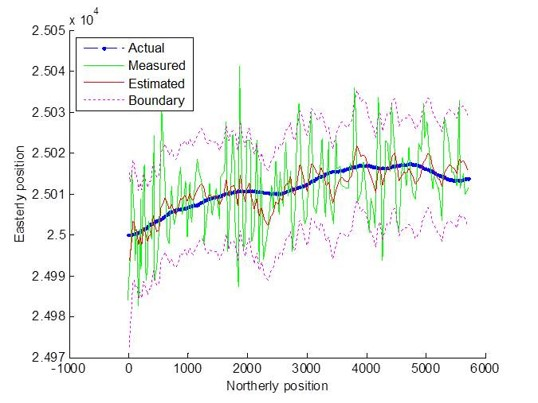
\includegraphics[width=0.9\textwidth]{localization_methods/ukf}
	\caption[Unscented Kalman Filter]{Unscented Kalman Filter\protect\footnotemark}
	\label{fig:localization-methods_ukf}
\end{figure}
\footnotetext{\url{http://www.lzcheng.com/courseworks/kalmanfilter}}
%}


\subsubsection{Perfect Match}

The Perfect Match \cite{Lauer2006a,Pinto1963} is an efficient self-localization algorithm that is largely used in the Robocup Robotic Soccer Mid Size League. Its main goal is to minimize the localization error by carefully analyzing the know map and selecting the most probable current position using a gradient descent approach. To improve tracking accuracy, the algorithm also uses a stochastic weighted approach.

With the proper configuration, it can achieve a localization accuracy similar to the particle filter, while using about ten times less computations.

An example of the position estimation can be seen in the figures below. \Cref{fig:localization-methods_pm-1} shows the probable locations when the robot detects a line on the floor, and \cref{fig:localization-methods_pm-2} illustrates their associated errors (brighter areas indicate smaller error). By using a gradient descent, the most probable location was selected (black circle).

\begin{figure}[H]
	\centering
	\begin{minipage}[h]{.495\textwidth}
		\centering
		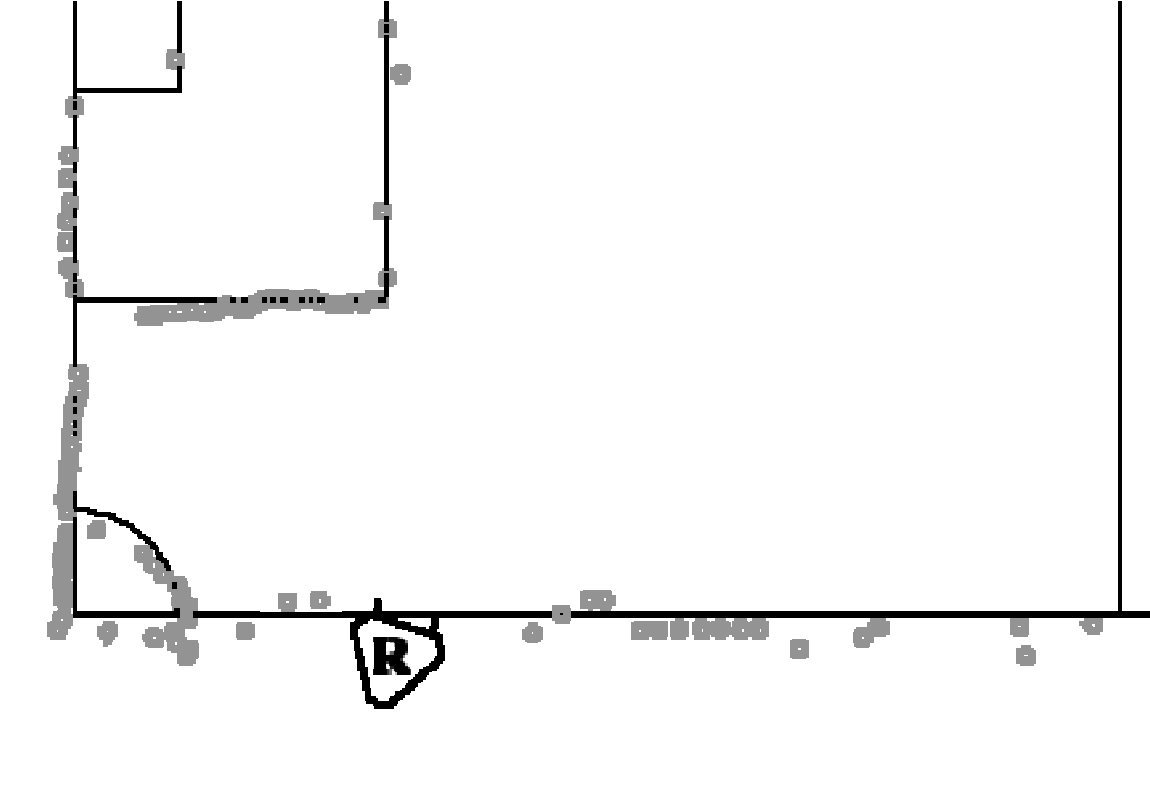
\includegraphics[width=\textwidth]{localization_methods/pm_1}
		\caption{Position estimates}
		\label{fig:localization-methods_pm-1}
	\end{minipage}\hfill
	\begin{minipage}[h]{.495\textwidth}
		\centering
		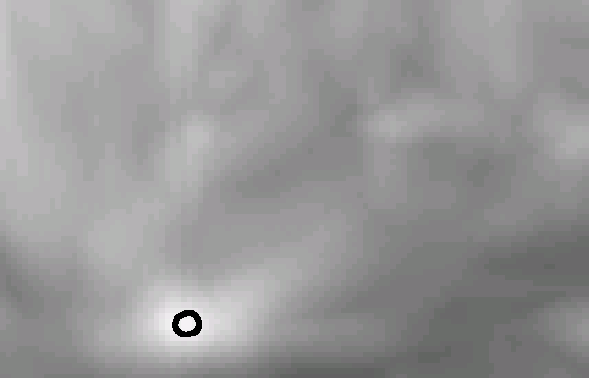
\includegraphics[width=\textwidth]{localization_methods/pm_2}
		\caption{Positions associated error}
		\label{fig:localization-methods_pm-2}
	\end{minipage}
\end{figure}


\subsection{\glsentryfirst{slam}}

\gls{slam} \cite{Thrun2002} is a very effective approach to either explore unknown environments or update a known map. It relies on both proprioceptive and exteroceptive methods to perform localization and mapping. It is also very useful to make the robot navigation more robust in dynamic environments, in which the topology of the world may change considerably over time.

There are numerous approaches to perform  \gls{slam} \cite{Tuna2012}. Some optimized for exploration and others for map improvement. For the exploration tasks, proprioceptive methods play a critical role, and are usually paired with probabilistic methods, such as Kalman filters, in order to reliably map the environment. For map correction and improvement, several probabilistic methods can be employed according to the precision required. For high accuracy 3D mapping, the \gls{icp} algorithm can be used to build accurate point clouds of the environment.



\section{Summary}

This chapter introduced several localization systems that can be used in different types of environments and with different degrees of accuracy. It started with the simple proprioceptive methods and then moved on to the more robust exteroceptive approaches.

Some techniques can be combined to improve the pose estimate or to make the localization more efficient to a particular type of environment.

For outside tasks, a \gls{gnss} approach can give accurate localization estimations with very little computation cost. On the other hand, indoor localization requires more advanced techniques in order to infer the current position based on the analysis of the robot surroundings. These techniques usually start with an estimation of the robot movement and then refine it with probabilistic or geometric methods.

\Cref{tab:localization-methods_overview-self-localization-approaches} presents an overview of the mentioned localization techniques.


\begin{sidewaystable}
	\caption{Overview of self-localization approaches}
	\tabulinesep = 0.9ex
	\centering
	\begin{tabu} { X[1.4,m,c] | X[m,c] X[m,c] X[m,c] X[m,c] X[6,m,c] }
		\rowfont{\bfseries\itshape} Method & Ideal environment & Accuracy & Operational cost & Computational cost & Notes \\
		\hline
		Odometry			& Any		& Low		& Low		& Low		& Position estimation is affected by cumulative errors \\
		Dead reckoning		& Any		& Low		& Low		& Low		& Pose estimation is affected by cumulative errors \\
		\gls{lidar}			& Any		& High		& Medium	& High		& Needs an auxiliary method to perform global localization \\
		\gls{radar}			& Any		& Medium	& High		& High		& Needs an auxiliary method to perform global localization \\
		\gls{sonar}			& Any		& Medium	& Medium	& High		& Needs an auxiliary method to perform global localization \\
		\gls{gnss}			& Outside	& Medium	& Low		& Low		& Requires a clear line of sight to at least 3 satellites \\
		Signal strength		& Any		& Low		& Low		& Low		& Requires an accurate model for the signal attenuation \\
		Celestial			& Outside	& Low		& Low		& Low		& Requires a clear view of the celestial objects and a nautical almanac \\
		Landmark			& Any		& Medium	& Low		& Medium	& Requires a database of landmarks \\
		\gls{icp}			& Indoors	& High		& Medium	& High		& Requires a detailed 3D representation of the environment \\
		\gls{mcl}			& Indoors	& Medium	& Medium	& Medium	& Inefficient for large areas \\
		Kalman filters		& Any		& Medium	& Low		& Low		& Useful to improve estimations of other methods \\
		Perfect Match		& Any		& Medium	& Low		& Low		& Not ideal for large or dynamic environments \\
		\gls{slam}			& Indoors	& Medium	& Medium	& High		& Adapts well to dynamic environments \\
	\end{tabu}
	\label{tab:localization-methods_overview-self-localization-approaches}
\end{sidewaystable}

\chapter{Relevant software / hardware technologies}\label{chap:relevant-sofware-hardware-technologies}



\section*{}

Robot self-localization in complex environments is a multidisciplinary problem that requires advanced computer software systems. In order to speed up the implementation and deployment of the localization system, several frameworks and libraries were used. Among the most important were \gls{ros} for the system architecture, \gls{pcl} for the point cloud processing and Gazebo for simulation and testing.



\section{\glsentrytext{ros}}

\begin{wrapfigure}{r}{0.25\textwidth}
	\centering
	\includegraphics*[width=0.24\textwidth]{relevant_sofware_hardware_technologies/ros_logo}
	\caption{\glsentrytext{ros} logo}
	\label{fig:relevant-sofware-hardware-technologies_ros-logo}
\end{wrapfigure}

\gls{ros}\footnote{\url{http://www.ros.org/}} \cite{Quigley2009} is a software framework designed to ease the development of robot systems. It provides seamless integration between hardware drivers and software modules, allowing a fast transition between simulation and deployment.

It's an open source project that offers a distributed computing framework with several core libraries and development tools that aims to speedup software prototyping, testing and deployment.


\subsection{Architecture}

The \gls{ros} architecture was designed from the beginning to be a distributed peer-to-peer software framework that could be deployed in several operating systems and implemented in a range of different programming languages. However, given that most of the \gls{ros} community prefers open source software, the Ubuntu\footnote{\url{http://www.ubuntu.com/}}] operating system is the main developing and testing environment, and as such, the recommended choice for \gls{ros} developers. Moreover, considering that robotics research requires software with both performance and maintainability at its core, the C++\footnote{\url{http://www.cplusplus.com/}} programming language is used in most of the available packages, along with Python\footnote{\url{https://www.python.org/}} and Java\footnote{\url{https://www.java.com}}.

Being a distributed computing framework, \gls{ros} relies in network connections and exchange of messages to perform the intended tasks. As such, its architecture was developed to follow a publish / subscribe pattern (\gls{ros} topics\footnote{\url{http://wiki.ros.org/Topics}}) and request and reply communication paradigm (\gls{ros} services\footnote{\url{http://wiki.ros.org/Services}} and actions\footnote{\url{http://wiki.ros.org/actionlib}}). This allows \gls{ros} nodes\footnote{\url{http://wiki.ros.org/Nodes}} (operating system processes) to be deployed in different computing platforms with ease and simplifies testing and exchange of software modules.

The next sections provide a more detailed description of the main \gls{ros} architecture concepts.


\subsubsection{Nodes}

\gls{ros} nodes are operating system processes that are part of the peer-to-peer communication graph. They are the fundamental building blocks of any \gls{ros} system and can be spread among several computing platforms.

In order to manage the communications between nodes, the \gls{ros} framework provides a master node (roscore\footnote{\url{http://wiki.ros.org/roscore}}) that uses \gls{xmlrpc} to maintain a communication graph of the system. This allows nodes to be started without knowing the location (\gls{ip} address and port) of the other nodes in the network and greatly simplifies their integration and exchange. Also, by using \gls{ros} launch files\footnote{\url{http://wiki.ros.org/roslaunch}} (\gls{xml} configuration files), the specification of a system communication data flow and configuration can be easily altered.

Besides handling communications, the master node also manages system configurations through the parameter server. This allows nodes to share and change the system configuration at runtime. However, given that the parameter server is usually queried only when a node starts up, the dynamic reconfigure\footnote{\url{http://wiki.ros.org/dynamic_reconfigure}} \gls{api} can be used instead, if it is necessary to change the configuration of a node when it is already running. This is achieved by providing a callback that is asynchronously called when a configuration change is requested.

The flexibility provided by \gls{ros} in both module integration and exchange can greatly speedup testing and deployment and the possibility of changing the configuration of the system at runtime and restart software modules individually (nodes) is very useful when implementing system supervisors and recovery behaviors.


\subsubsection{Nodelets}

A nodelet\footnote{\url{http://wiki.ros.org/nodelet}} is a special kind of node that aims to reduce the overhead of message exchange. This overhead can be significant when messages are very large, such as point clouds or video. To mitigate this problem, the nodelets exchange pointers to shared memory regions, instead of sending the entire messages between nodes.

To achieve this overhead reduction, some architecture changes are required. The most important being the use of threads instead of processes, and the creation of a superclass that all nodelets must inherit. This leads to the creation of plugin libraries for each nodelet instead of an executable for each node.

Another important change is the introduction of nodelet managers to allow loading and setup of nodelets in different threads inside the same process.

In terms of implementation, the transition from nodes to nodelets requires few code changes and can lead to a significant improvement of the overall system performance.


\subsubsection{Topics}

\gls{ros} topics are named communication buses that follow the publish / subscribe pattern. They provide a simple method for exchanging messages between nodes and allow the decoupling of information production and consumption. This is useful when there are multiple sources of the same information or there are multiple consumers that are interested in processing the same data for different purposes. Moreover, this communication architecture allows to log and replay the exchanged messages, which can be helpful to test different algorithms with the same data.

Currently, topics can use either the \gls{tcp} or \gls{udp} protocols to exchange messages. The \gls{tcp} implementation is used by default and creates a bidirectional channel between each producer and subscriber while guaranteeing the delivery of all messages. The \gls{udp} implementation uses an unreliable and stateless transport approach, in which a subscriber listens to a given broadcast address, and has no guarantee that will receive all messages. As such, \gls{tcp} should be used when all messages must be processed, and \gls{udp} should be considered when the latency and the \gls{tcp} overhead are important issues.


\subsubsection{Services}

\gls{ros} services are named communication buses that follow the request and reply paradigm, in which a node asks for a given service and receives a response according to the data that was sent in the request message and the state of the service node. They are useful to query other nodes state or to request the execution of some behavior / action.


\subsubsection{Actions}

\gls{ros} actions are a special kind of service in which the progress of the request can be queried. They are very useful when the request might take a long time, and gives the caller the necessary information to supervise the execution of the request and if necessary, terminate its execution.


\subsection{Build system}

The latest \gls{ros} build system is named catkin\footnote{\url{http://wiki.ros.org/catkin}}, and is the successor of the original rosbuild\footnote{\url{http://wiki.ros.org/rosbuild}} system. It combines CMake\footnote{\url{http://www.cmake.org/}} macros and Python scripts to allow building multiple dependent projects at the same time. It is a cross-platform build system, organized in packages and meta-packages (group of packages). Each package is a software module that can produce libraries or binaries from source code.

Catkin was designed to deal with complex build configurations, which in the case of \gls{ros} packages involves a considerable amount of build dependencies for each project. As such, catkin provides a build system that can easily find, build and link both \gls{ros} and system dependencies. Moreover, it provides install targets to allow faster code releases and simplifies builds from source for the final users.

Other useful features of the catkin build system are the concepts of workspace and overlays. Catkin uses a workspace with out-of-source builds to keep the source code separate from the build files. This allows the code directory structure to be clean of compiler generated files that are platform dependent. Moreover, it simplifies the concurrent usage of packages (overlay), because catkin gives priority to workspace packages (in relation to system packages). This is particularly useful when it is necessary to modify and test some package that has been released and is installed in the system (without having to uninstall the stable release of that package).

Finally, catkin is a cross-platform build system that can be used to build other projects that use CMake and are not related to \gls{ros}.


\subsection{Development tools}

\gls{ros} provides several development tools that allow introspection and visualization of the system state. They are very useful for testing, debugging and profiling.

The next sections give an overview of the most important \gls{ros} tools that are currently available.


\subsubsection{Graphical User Interface tools}

The \gls{ros} development tools that have graphical user interfaces are aggregated in the rqt framework\footnote{\url{http://wiki.ros.org/rqt}}, and are loaded as plugins at runtime (some can be started as standalone applications).

Currently there is plugins to visualize sensor data (rviz\footnote{\url{http://wiki.ros.org/rviz}}); introspect the contents of topics; log and replay \gls{ros} messages (rosbag\footnote{\url{http://wiki.ros.org/rosbag}}); display node, package and coordinate systems graphs; list and filter debug messages; change configuration of running nodes (dynamic reconfigure); monitor nodes memory and processor usage and much more.


\subsubsection{Command line tools}

The \gls{ros} command line tools\footnote{\url{http://wiki.ros.org/ROS/CommandLineTools}} are split across several executables and can be used for advanced introspection (rosnode, rostopic and rosservice), system configuration (rosparam), package building and management (catkin, rosdep and rosinstall) and also to search \gls{ros} message types documentation (rosmsg and rossrv).

Finally, it is available a diagnostics tool (roswtf), that can detect packages / dependencies issues and configuration problems.



\section{\glsentrytext{pcl}}

\begin{wrapfigure}{r}{0.25\textwidth}
	\centering
	\includegraphics*[width=0.24\textwidth]{relevant_sofware_hardware_technologies/pcl_logo}
	\caption{\glsentrytext{pcl} logo}
	\label{fig:relevant-sofware-hardware-technologies_pcl-logo}
\end{wrapfigure}

The \gls{pcl}\footnote{\url{http://pointclouds.org/}} \cite{Rusu2011} is an open source project that provides algorithms for processing point clouds. These algorithms can be used to filter and register point clouds as well as perform object segmentation, recognition and tracking.

\Cref{fig:relevant-sofware-hardware-technologies_pcl-dependency-graph} gives an overview of the main modules currently available in \gls{pcl}.

%\afterpage{
\begin{figure}[H]
	\centering
	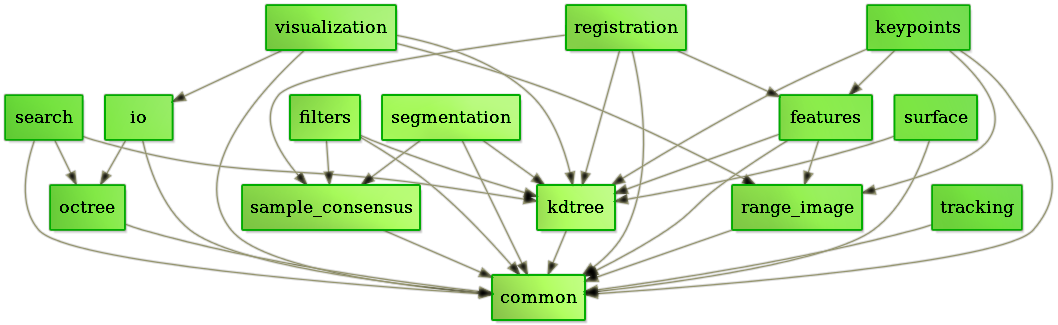
\includegraphics[width=\textwidth]{relevant_sofware_hardware_technologies/pcl_dependency_graph}
	\caption[\glsentrydesc{pcl}]{\glsentrydesc{pcl}\protect\footnotemark}
	\label{fig:relevant-sofware-hardware-technologies_pcl-dependency-graph}
\end{figure}
\footnotetext{\url{http://pointclouds.org/about/}}
%}

\clearpage



\section{Gazebo}

\begin{wrapfigure}{r}{0.25\textwidth}
	\centering
	\includegraphics*[width=0.24\textwidth]{relevant_sofware_hardware_technologies/gazebo_logo}
	\caption{Gazebo logo}
	\label{fig:relevant-sofware-hardware-technologies_gazebo-logo}
\end{wrapfigure}


Gazebo\footnote{\url{http://gazebosim.org/}} is a 3D multi-robot simulator capable of generating hardware sensor data for different kinds of robots while providing a realistic environment with physics simulation and 3D visualization. It is very useful to speedup testing of algorithms with different types of robots and environments.

\Cref{fig:relevant-sofware-hardware-technologies_gazebo-ros-integration} shows how Gazebo can be used instead of a real robot, without requiring any implementation code modification (because it implements the same \gls{ros} interfaces that the hardware drivers use).

%\afterpage{
\begin{figure}[ht]
	\centering
	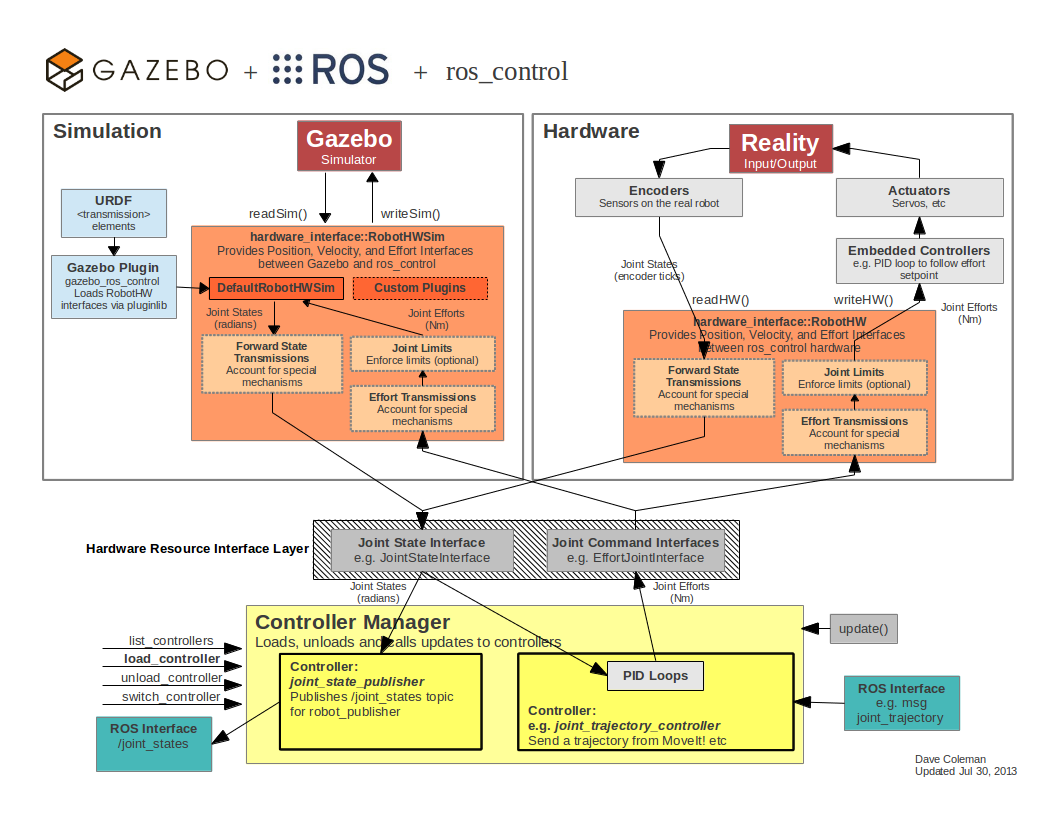
\includegraphics[width=0.8\textwidth]{relevant_sofware_hardware_technologies/gazebo_ros_integration}
	\caption[Integration of \glsentrytext{ros} and Gazebo]{Integration of \glsentrytext{ros} and Gazebo\protect\footnotemark}
	\label{fig:relevant-sofware-hardware-technologies_gazebo-ros-integration}
\end{figure}
\footnotetext{\url{http://gazebosim.org/tutorials?tut=ros_control}}
%}

\clearpage



\section{Point cloud acquisition}

Point clouds can be retrieved with a wide range of sensors with varying levels of precision and assembly time \cite{Sansoni2009}. The next sections provide a brief overview of the three main groups of methods capable of generating point clouds.


\subsection{Structured light methods}

Structured light methods can retrieve 3D geometry from images by projecting a known pattern into the environment and analyzing its deformation (example in \Cref{fig:relevant-sofware-hardware-technologies_structured-light}). They can achieve sample rates of 30 Hz, and besides 3D geometry they can also retrieve color information.

\begin{figure}[H]
	\centering
	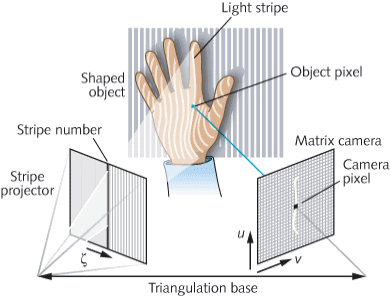
\includegraphics[width=0.5\textwidth]{relevant_sofware_hardware_technologies/structured_light}
	\caption[Structured light system diagram]{Structured light system diagram\protect\footnotemark}
	\label{fig:relevant-sofware-hardware-technologies_structured-light}
\end{figure}
\footnotetext{{\scriptsize \url{http://www.laserfocusworld.com/articles/2011/01/lasers-bring-gesture-recognition-to-the-home.html}}}


The Kinect 2\footnote{\url{http://www.microsoft.com/en-us/kinectforwindows/}} (seen in \cref{fig:relevant-sofware-hardware-technologies_kinect2}) is an example of a structured light system and can achieve measurements with millimeter accuracy for objects close to the sensor. Another similar sensor is Structure IO\footnote{\url{http://structure.io/}} which is intended for mobile devices and can be seen in \cref{fig:relevant-sofware-hardware-technologies_structure-io}.

%\afterpage{
\begin{savenotes}
\begin{figure}[H]
	\centering
	\begin{minipage}[h]{.47\textwidth}
		\centering
		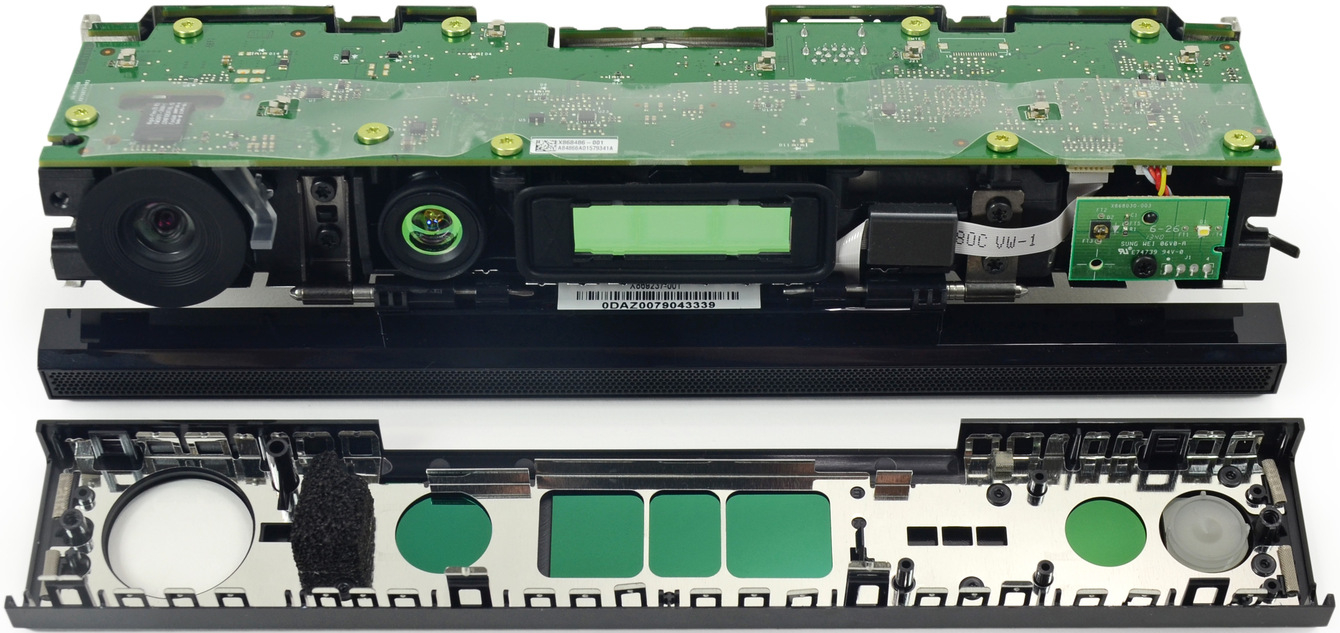
\includegraphics[width=\textwidth]{relevant_sofware_hardware_technologies/kinect2}
		\caption[Kinect 2 sensor]{Kinect 2 sensor\protect\footnotemark}
		\label{fig:relevant-sofware-hardware-technologies_kinect2}
	\end{minipage}\hfill
	\footnotetext{\scriptsize \url{https://www.ifixit.com/Teardown/Xbox+One+Kinect+Teardown/19725}}
	\begin{minipage}[h]{.47\textwidth}
		\centering
		\includegraphics*[width=0.7\textwidth]{relevant_sofware_hardware_technologies/structure_io}
		\caption[Structure IO sensor]{Structure IO sensor\protect\footnotemark}
		\label{fig:relevant-sofware-hardware-technologies_structure-io}
	\end{minipage}
	\footnotetext{\scriptsize \url{http://structure.io/press}}
\end{figure}
\end{savenotes}
%}



\subsection{\glsentrydesc{tof} methods}\label{sec:relevant-sofware-hardware-technologies_tof-methods}

\gls{tof} or \gls{toa} methods can be used to calculate distances based on the amount of time that a given wave takes from the moment it is created to the moment it is received. By assembling a large amount of sensor readings a 3D representation of the environment can be achieved.

Since these systems rely on active interaction with the environment, they can be used without being affected by lighting interferences. Nevertheless, they should take in consideration the conditions in which the waves propagate and also the geometry of the environment, because it can affect the path that the waves take, and as a result, can lead to the decrease of precision in the measurements.


\subsubsection{Light waves}

Light waves generated with lasers can estimate distances with millimeter accuracy at long ranges (system operation overview in \cref{fig:relevant-sofware-hardware-technologies_time-of-flight}) and their sensors usually have a low sample rate (below 20 Hz). Systems like \gls{lidar} (2D sensor example in \cref{fig:relevant-sofware-hardware-technologies_sick-nav-350} and for 3D in \cref{fig:relevant-sofware-hardware-technologies_velodyne-hdl-64e}) take advantage of this fact and can be used to obtain a very detailed 3D point cloud of the environment (like the one showed in \cref{fig:relevant-sofware-hardware-technologies_lidar-scan}). Moreover, some \glspl{lidar} can also capture the environment reflectivity / intensity besides their 3D geometry. On the other hand, \gls{tof} cameras (example in \cref{fig:relevant-sofware-hardware-technologies_mesa-sr4000}) have a very high sample rate (30 Hz or even higher), but have much more measurement error (greater than 1 cm). However, these methods allow the mapping of the environment with low latency, which can be a critical requirement in robots that must react very fast to changes in their surroundings, such as autonomous cars \cite{Moras2010}.

\begin{figure}[H]
	\centering
	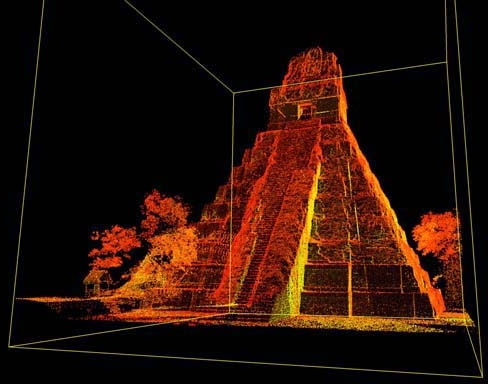
\includegraphics[width=0.6\textwidth]{relevant_sofware_hardware_technologies/lidar_scan}
	\caption[\glsentrytext{lidar} scan]{\glsentrytext{lidar} scan\protect\footnotemark}
	\label{fig:relevant-sofware-hardware-technologies_lidar-scan}
\end{figure}
\footnotetext{\url{http://blogs.scientificamerican.com/cocktail-party-physics/2012/03/12/l-is-for-lidar/}}


%\afterpage{
\begin{savenotes}
\begin{figure}[H]
	\centering
	\begin{minipage}[h]{.47\textwidth}
		\centering
		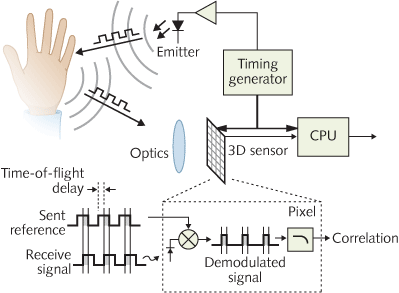
\includegraphics[width=0.8\textwidth]{relevant_sofware_hardware_technologies/time_of_flight}
		\caption[\glsentrydesc{tof} system diagram]{\glsentrydesc{tof} system diagram\protect\footnotemark}
		\label{fig:relevant-sofware-hardware-technologies_time-of-flight}
	\end{minipage}\hfill
\footnotetext{\url{http://www.laserfocusworld.com/articles/2011/01/lasers-bring-gesture-recognition-to-the-home.html}}
	\begin{minipage}[h]{.47\textwidth}
		\centering
		\includegraphics*[width=0.53\textwidth]{relevant_sofware_hardware_technologies/mesa_sr4000}
		\caption[Mesa SR4000 sensor]{Mesa SR4000 sensor\protect\footnotemark}
		\label{fig:relevant-sofware-hardware-technologies_mesa-sr4000}
	\end{minipage}
	\footnotetext{\scriptsize \url{http://www.mesa-imaging.ch/products/product-overview/}}
\end{figure}
\end{savenotes}
%}


%\afterpage{
\begin{savenotes}
\begin{figure}[H]
	\centering
	\begin{minipage}[h]{.47\textwidth}
		\centering
		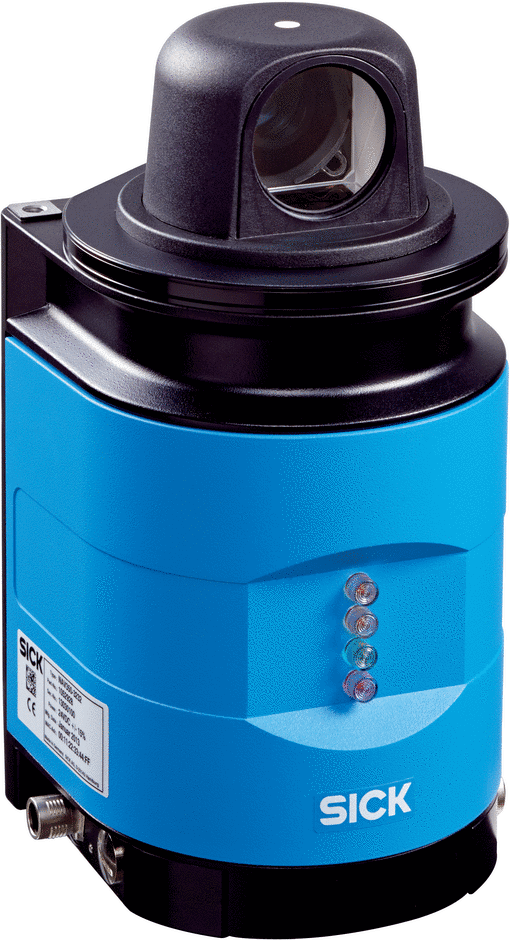
\includegraphics[width=0.4\textwidth]{relevant_sofware_hardware_technologies/sick_nav_350}
		\caption[2D SICK NAV 350 sensor]{2D SICK NAV 350 sensor\protect\footnotemark}
		\label{fig:relevant-sofware-hardware-technologies_sick-nav-350}
	\end{minipage}\hfill
\footnotetext{\url{https://www.sick.com/de/en/detection-and-ranging-solutions/2d-laser-scanners/nav/nav350-3232/p/p256041}}
	\begin{minipage}[h]{.47\textwidth}
		\centering
		\includegraphics*[width=0.67\textwidth]{relevant_sofware_hardware_technologies/velodyne_hdl_64e}
		\caption[3D Velodyne HDL-64E sensor sensor]{3D Velodyne HDL-64E sensor\protect\footnotemark}
		\label{fig:relevant-sofware-hardware-technologies_velodyne-hdl-64e}
	\end{minipage}
	\footnotetext{\scriptsize \url{http://www.velodynelidar.com/lidar/hdlproducts/hdl64e.aspx}}
\end{figure}
\end{savenotes}
%}


\subsubsection{Radio waves}

Similar to \gls{lidar}, radio waves can be used to calculate distances using the \gls{tof} technique. Systems like \gls{radar} provide an effective way to calculate the distance, altitude, direction and speed of objects that can be used as landmarks in navigation.

Like any electromagnetic wave localization method, it must take in consideration ambient interferences and even jamming, in order to validate the obtained measures. Moreover, some types of materials with a given geometric configuration might be invisible to \gls{radar}, and as such, critical localization systems might have to employ some additional techniques to ensure the correct mapping of the robot surroundings.

Since \gls{radar} has a less focused beam than \gls{lidar}, it can have considerable less accuracy, as can be seen in \cref{fig:relevant-sofware-hardware-technologies_radar-scan}. Nevertheless, it can be an effective method to avoid obstacles \cite{Wu2007}.


%\afterpage{
\begin{savenotes}
\begin{figure}[H]
	\centering
	\begin{minipage}[h]{.47\textwidth}
		\centering
		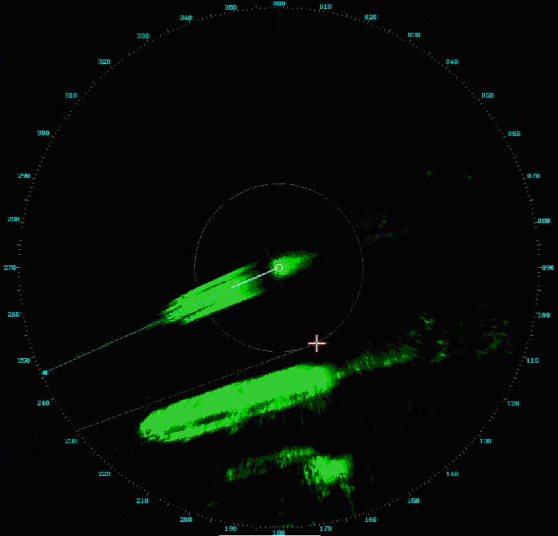
\includegraphics[width=0.9\textwidth]{relevant_sofware_hardware_technologies/radar_scan}
		\caption[\glsentrytext{radar} scan of two ships]{\glsentrytext{radar} scan of two ships\protect\footnotemark}
		\label{fig:relevant-sofware-hardware-technologies_radar-scan}
	\end{minipage}\hfill
	\footnotetext{\scriptsize \url{http://www.sintef.no/Projectweb/STSOps/News/Operational-Aspects-on-Decision-making-in-STS-Lightering}}
	\begin{minipage}[h]{.47\textwidth}
		\centering
		\includegraphics*[width=0.7\textwidth]{relevant_sofware_hardware_technologies/radar_qt50r}
		\caption[QT50R-AFH \glsentrytext{radar} sensor]{QT50R-AFH \glsentrytext{radar} sensor\protect\footnotemark}
		\label{fig:relevant-sofware-hardware-technologies_radar-qt50r}
	\end{minipage}
	\footnotetext{\scriptsize \url{http://www.bannerengineering.com/en-US/products/8/Sensors/658/Radar-Sensors/617/R-GAGE-QT50R-AFH-Adjustable-Field\%2C-High-Sensitivity-Sensor/}}
\end{figure}
\end{savenotes}
%}



\subsubsection{Sound waves}

Another type of 3D sensor that can be used to map under water environments relies in the acoustic analysis of the reflections of sounds in the surrounding objects. Like the previous methods, \gls{sonar} can actively scan the environment to calculate the locations of the objects using a \gls{tof} technique (as can be seen in \cref{fig:relevant-sofware-hardware-technologies_sonar-scan}). Although this method is usually applied to underwater mapping, it can also be used in other sound propagation environments, such as air \cite{Guarato2013}.

%\afterpage{
\begin{savenotes}
\begin{figure}[H]
	\centering
	\begin{minipage}[h]{.47\textwidth}
		\centering
		\includegraphics*[width=0.9\textwidth]{relevant_sofware_hardware_technologies/sonar_scan}
		\caption[\glsentrytext{sonar} scan of two ships]{\glsentrytext{sonar} scan of two ships\protect\footnotemark}
		\label{fig:relevant-sofware-hardware-technologies_sonar-scan}
	\end{minipage}
	\footnotetext{\scriptsize \url{http://stellwagen.noaa.gov/maritime/palmercrary.html}}
	\begin{minipage}[h]{.47\textwidth}
		\centering
		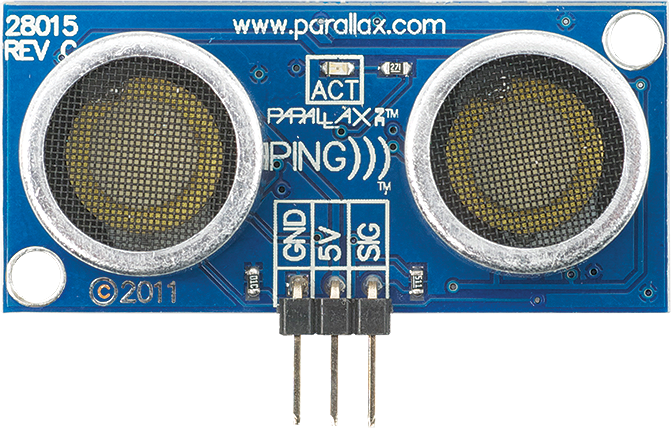
\includegraphics[width=\textwidth]{relevant_sofware_hardware_technologies/sonar_ping}
		\caption[\glsentrytext{sonar} sensor]{\glsentrytext{sonar} sensor\protect\footnotemark}
		\label{fig:relevant-sofware-hardware-technologies_sonar-ping}
	\end{minipage}\hfill
	\footnotetext{\scriptsize \url{http://www.parallax.com/product/28015}}
\end{figure}
\end{savenotes}
%}


\subsection{Stereo vision}

Stereo vision systems (example in \cref{fig:relevant-sofware-hardware-technologies_stereo-cameras}) can generate 3D representations of the environment by comparing the displacement of corresponding points in the two ambient images (\cref{fig:relevant-sofware-hardware-technologies_stereo-vision} gives an overview of such a system). This can be achieved because the relative position of the cameras is known. As such, points farther away will have smaller displacement between images than points closer to the cameras. In the end, a disparity image is obtained, that can then be converted to a point cloud representation of the environment.

Given that the accuracy of the disparity image relies heavily in the correct matching of points between the left and right image, some stereo vision systems employ active observation by projecting a pattern into the environment in order to refine the point matching (example of hardware setup in \cref{fig:relevant-sofware-hardware-technologies_pr2-active-stereo}). This can significantly improve the accuracy if the environment has a lot of smooth surfaces with homogeneous colors.


\begin{figure}[H]
	\centering
	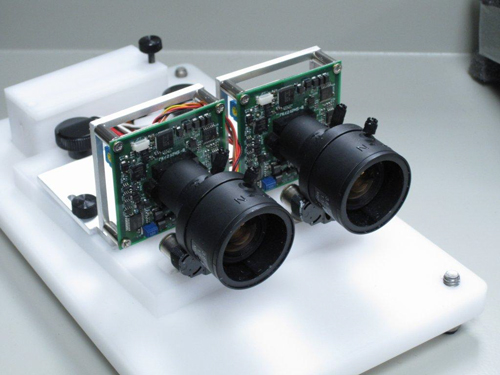
\includegraphics[width=0.55\textwidth]{relevant_sofware_hardware_technologies/stereo_cameras}
	\caption[Stereo vision system]{Stereo vision system \cite{Kaczurba2013}}
	\label{fig:relevant-sofware-hardware-technologies_stereo-cameras}
\end{figure}


\begin{figure}[H]
	\centering
	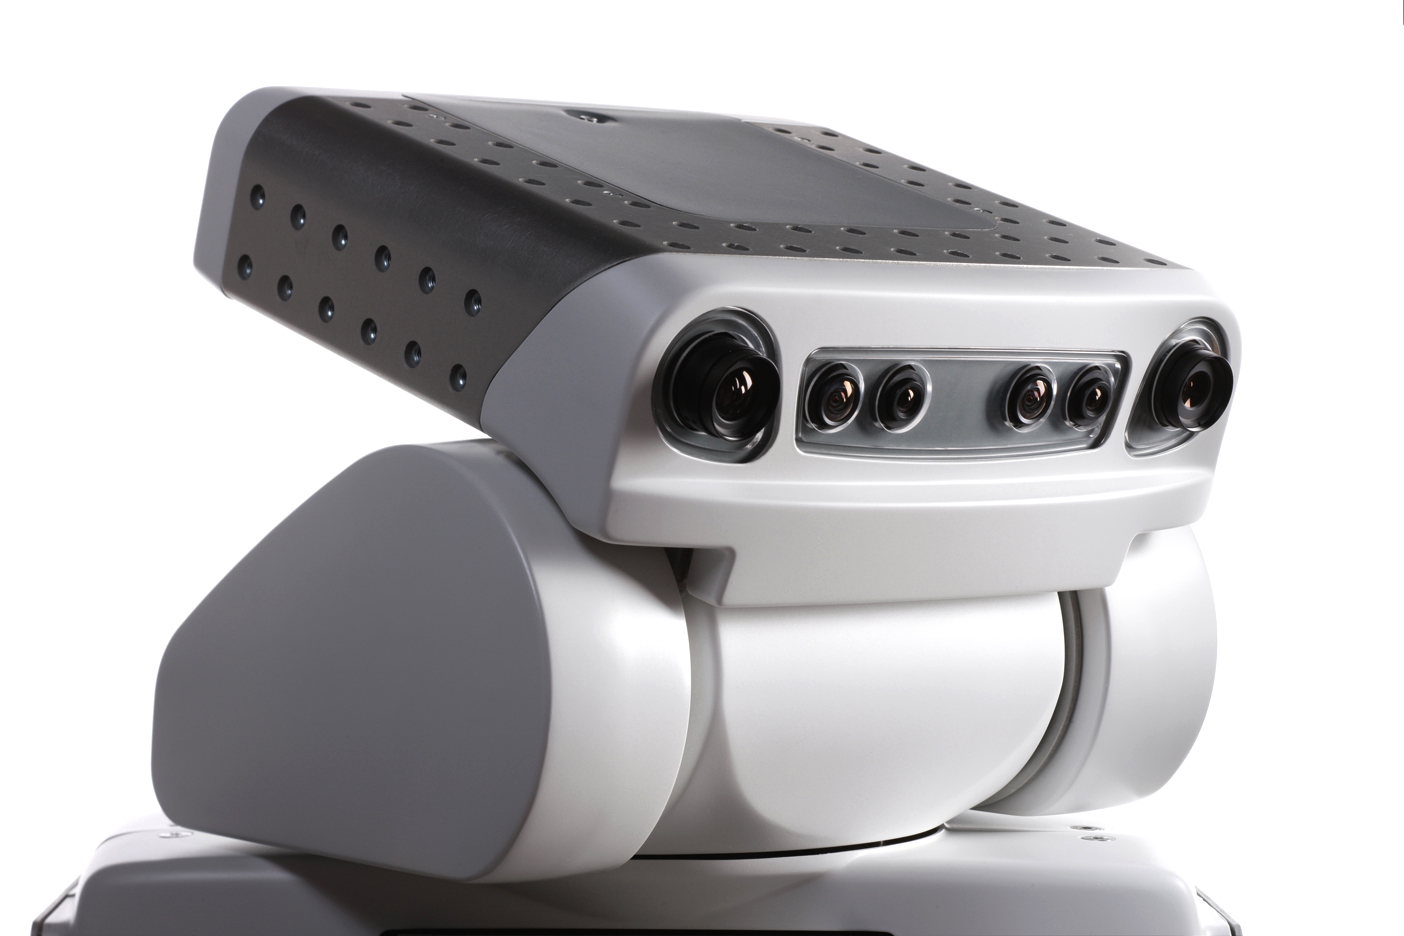
\includegraphics[width=0.55\textwidth]{relevant_sofware_hardware_technologies/pr2_active_stereo}
	\caption[PR2 head capable of active stereo vision]{PR2 head capable of active stereo vision\protect\footnotemark}
	\label{fig:relevant-sofware-hardware-technologies_pr2-active-stereo}
\end{figure}
\footnotetext{\url{https://www.willowgarage.com/pages/pr2/overview}}


\begin{figure}[hb]
	\centering
	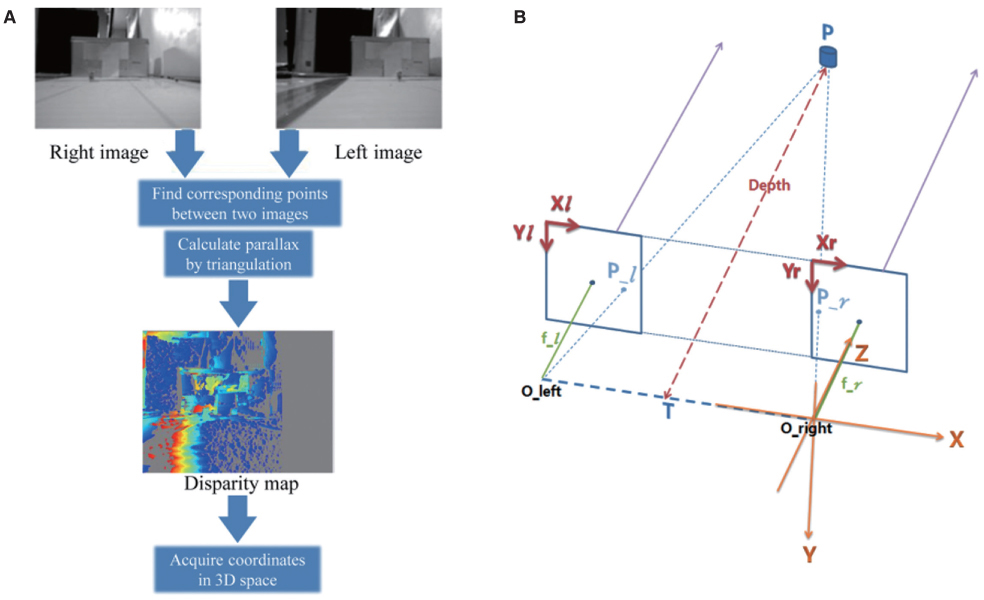
\includegraphics[width=\textwidth]{relevant_sofware_hardware_technologies/stereo_vision}
	\caption[Stereo vision overview]{Stereo vision overview \cite{Yang2014}}
	\label{fig:relevant-sofware-hardware-technologies_stereo-vision}
\end{figure}


\chapter{Localization system} \label{chap:localization-system}



\section*{}

FF



\section{FF}

FF

\chapter{Localization system evaluation} \label{chap:localization-system-evaluation}



\section*{}

FF



\section{FF}

FF

\chapter{Conclusions} \label{chap:conclusions-and-future-work}



\section*{}

The proposed localization system is able to maintain pose tracking with less 1-2 centimeters of translation error and less than a 1-3 degrees of rotation error (in 3 and 6 DoF respectively) with the sensors moving at several velocities even in cluttered and dynamic environments. Moreover, when tracking is lost or no initial pose is given, the system is able to find a valid global pose estimate by switching to more robust registration algorithms that use feature matching. This approach achieved fast pose tracking and reliable initial pose estimation while also providing the set of the accepted initial poses before registration refinement, which can be very valuable information for a navigation supervisor when the robot is in an ambiguous region that can be registered in similar zones of the known map. The system also allows dynamic reconfiguration of the number of laser scans to assemble in order to mitigate laser measurement errors and can adapt its rate of operation according to the robot estimated velocity.

The sub-centimeter accuracy achieved by the proposed localization system along with the dynamic map update capability and the need of no artificial landmarks / ambient modifications will allow the fast deployment of mobile robots capable to operate safely and accurately in cluttered environments.



\section{Main contributions}

The following list gives an overview of the main contributions of the presented work:

\begin{itemize}
	\item A \gls{lidar} assembler\footnote{\url{https://github.com/carlosmccosta/laserscan_to_pointcloud}} capable of:
	\begin{itemize}
		\item Merging measurements from several sensors
		\item Dynamic adjust its configurations based on the speed of the robot in order to merge more scans when the robot is moving slower
		\item Use spherical linear interpolation to reduce scan deformation
		\item Emulate a 3D sensor when the \gls{lidar} is mounted on a tilting platform
	\end{itemize}

	\item An localization system\footnote{\url{https://github.com/carlosmccosta/dynamic_robot_localization}} that:
	\begin{itemize}
		\item Is efficient, modular and extensible to new 3/6 \gls{dof} algorithms
		\item Can dynamically and incrementally update the localization map
		\item Provides the set of acceptable initial poses when reseting tracking (useful for localization supervisors)
		\item Gives several localization quality metrics such as percentage, \gls{rmse} and angular distribution of the correctly registered points
		\item Gives the possibility to use 3 different point cloud registration algorithms based on the tracking state (normal tracking, tracking recovery, initial pose estimation)
	\end{itemize}

	\item Development of a testing infrastructure to automate the collection, analysis and generation of localization results

	\item 3 \gls{dof} Localization datasets\footnote{\url{https://github.com/carlosmccosta/dynamic_robot_localization_tests}}:
	\begin{itemize}
		\item 4 datasets with subcentimeter ground truth in static and dynamic environments using a robot moving at different speeds
		\item 6 Gazebo and 6 Stage simulation datasets
		\item Improvement of external 3/6 \gls{dof} datasets (ground truth time synchronization and laser transformations calibration)
	\end{itemize}

	\item Test of the localization system on public datasets and comparison with:
	\begin{itemize}
		\item Ground truth systems from three different testing environments
		\item Widely used localization systems (\gls{amcl} and ethzasl-icp-mapper)
		\item Well known \gls{slam} system (GMapping)
	\end{itemize}
 	
	\item In the context of the \gls{carlos} project:
	\begin{itemize}
		\item The robot hardware configuration proved adequate for the intended tasks and environment
		\item The 3 \gls{dof} localization system was able to run in real time on the low computational power on-board computer
	\end{itemize}
\end{itemize}



\section{Future work}

The current implementation of the self-localization system can be further improved with \gls{gpu} support \cite{Tamaki2010} in order to achieve higher update rates in 6 \gls{dof} and also with loop closing algorithms \cite{Grisetti2012} in order to become a complete \gls{slam} system and allow the creation of accurate maps of very large environments. Moreover, it could be extended to support image based localization \cite{Labb2014} and semantic perception and mapping of the environment \cite{Santos2013}.





%---------------------------------------------------------------------------------------------------
% Appendixes, bibliography and index
%---------------------------------------------------------------------------------------------------

\appendix
\chapter{Appendix 1} \label{app:appendix1}



\section*{}

FF



\section{FF}

FF


\PrintBib{references/references}
%\PrintIndex


\end{document}
